\documentclass[review]{elsarticle}

\usepackage{lineno,hyperref}
\modulolinenumbers[5]

\journal{Journal of \LaTeX\ Templates}

%%%%%%%%%%%%%%%%%%%%%%%
%% Elsevier bibliography styles
%%%%%%%%%%%%%%%%%%%%%%%
%% To change the style, put a % in front of the second line of the current style and
%% remove the % from the second line of the style you would like to use.
%%%%%%%%%%%%%%%%%%%%%%%

%% Numbered
%\bibliographystyle{model1-num-names}

%% Numbered without titles
%\bibliographystyle{model1a-num-names}

%% Harvard
%\bibliographystyle{model2-names.bst}\biboptions{authoryear}

%% Vancouver numbered
%\usepackage{numcompress}\bibliographystyle{model3-num-names}

%% Vancouver name/year
%\usepackage{numcompress}\bibliographystyle{model4-names}\biboptions{authoryear}

%% APA style
%\bibliographystyle{model5-names}\biboptions{authoryear}

%% AMA style
%\usepackage{numcompress}\bibliographystyle{model6-num-names}

%% `Elsevier LaTeX' style
\bibliographystyle{elsarticle-num}
%%%%%%%%%%%%%%%%%%%%%%%

\begin{document}

\begin{frontmatter}

\title{Multi-modal fusion for violent scene detection in Hollywood movies}
\tnotetext[mytitlenote]{Fully documented templates are available in the elsarticle package on \href{http://www.ctan.org/tex-archive/macros/latex/contrib/elsarticle}{CTAN}.}

%% Group authors per affiliation:
\author{Elsevier\fnref{myfootnote}}
\address{Radarweg 29, Amsterdam}
\fntext[myfootnote]{Since 1880.}

%% or include affiliations in footnotes:
\author[mymainaddress,mysecondaryaddress]{Elsevier Inc}
\ead[url]{www.elsevier.com}

\author[mysecondaryaddress]{Global Customer Service\corref{mycorrespondingauthor}}
\cortext[mycorrespondingauthor]{Corresponding author}
\ead{support@elsevier.com}

\address[mymainaddress]{1600 John F Kennedy Boulevard, Philadelphia}
\address[mysecondaryaddress]{360 Park Avenue South, New York}

\begin{abstract}
Violent scene detection (VSD) is a challenging problem because of the heterogeneous content, large variations in video quality, high semantic meaning of the concepts. In the last few years, combining multiple features from multi-modalities is proven as an effective strategy for a wide range of video classification tasks and almost existing works have focused on general multimedia event detection (MED), the specific event detection like VSD has been comparatively less studied. In this work, we try to study the value of multi features and combination of these features for VSD in Hollywood movies. We rigorously analyze and combine a set of low-level features and deep learning feature that capture appearance, color, texture, motion and audio in videos. We also evaluate the utility of mid-level visual information obtained from detecting related violent concepts. Experiments are performed on MediaEval VSD 2014 dataset, made publicly available. Results show the performance of visual and motion features are better than audio features. The performance of mid-level features was nearly as good as that of low-level visual features. Experiments with a number of fusion methods show that all single features are complementary and help to improve overall performance. This study also provides an empirical foundation for selecting feature sets that are capable of dealing with heterogeneous content data as violent scenes in movies.
\end{abstract}

\begin{keyword}
violent scene detection,video retrieval,multi-modal fusion,multiple features
\end{keyword}

\end{frontmatter}

\linenumbers

\section{Introduction}

\begin{figure}[!b]
	\centering
	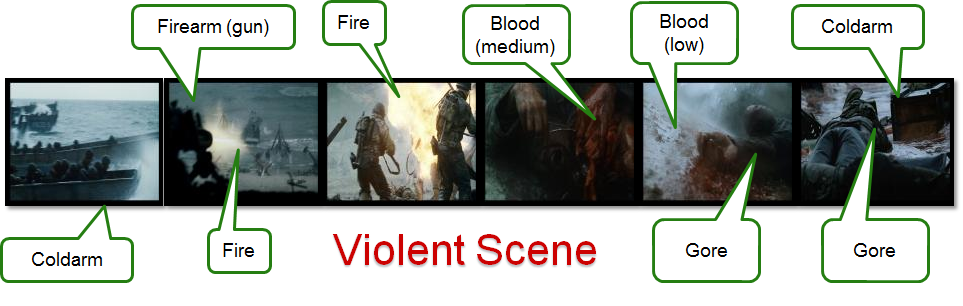
\includegraphics[width=1\linewidth]{Images/ViolentScene.png}
	\caption{Following the violent definition in \cite{demarty2014benchmarking}, this is an example of a violent scene in Saving Private Ryan Movie because it contains physical violence or accident resulting (fighting scene: boats approaching, guns shooting, fire guns shooting,..) in human injury or pain (blood and gory, dead soldiers)}
	\label{fig:exampleVS}
\end{figure}

Nowadays, the movie industry generates thousands of movies each year. However, not all movies are suitable for young people (especially children, teenagers, e.g.) to watch, because they might have violent contents.   The research from University of Pittsburgh \footnote{http://www.ocd.pitt.edu/Files/PDF/Parenting/TvAndMovieViolence.pdf} reports that watching violence in movies or TV programs tends to make children more aggressive and leads to unhealthy attitudes. It is crucial to have violent scene detection (VSD) system which enables the parents to choose movies that are suitable for their children. More general, for content provider, the violent scene detection technique can be used to assist in movie rating; for general end users, it can block the violent content in client terminal devices. 

% Violent scene detection in the movie is a very challenging problem, particularly because the movies contain the heterogeneous content, have large variations in quality. Because violence concept has a high semantic meaning, violent segments in video can contain the huge collection of {\bf affective content} which refers to the characterization of violence concept, such as blood,  gun, cold arm, firearm;  {\bf actions} such as fighting, running, shooting, etc.; {\bf activities} such as car chase, boat chase, etc.; {\bf scenes} such as gory scene, overcast, scene etc.; {\bf sound} such as gun shot, scream, explosion, etc.; and their strictly spatial/temporal relationships (for example: a scene with two man are fighting first and after that they get injury or pain). Besides that, movies often have a lot of effects, scene transition techniques which are heavily edited by the producers.  Figure~\ref{fig:exampleVS}\, shown an example of violent scene in Hollywood movie.

Detecting violent scene is a challenging task mainly due to the large variation of violence concept and the semantic gap between the concept and low-level features provided in the media. To capture violence insights, multiple features (e.g. global or local static visual features, motion-based featuers, and audio features) are extracted for learning and prediction. Besides, to narrow the semantic gap, a set of various mid-level concepts and their spatial temporal relationships can be used to characterize violence e.g. {\bf object-based concepts}: blood,  gun, cold arm, firearm; {\bf action-based concepts}: fighting, running, shooting, etc.; {\bf activity-based concepts}: car chase, boat chase; {\bf scene-based concepts}: gory scene, overcast, scene; {\bf sound-based concepts} such as gun shot, scream, explosion. Figure~\ref{fig:exampleVS} demonstrate an example of violent scene in a Hollywood movie. However, how to precisely detect mid-level concepts and efficiently utilize their relationships is yet another challenging and unsolved problem.
\begin{figure}[!b]
	\centering
	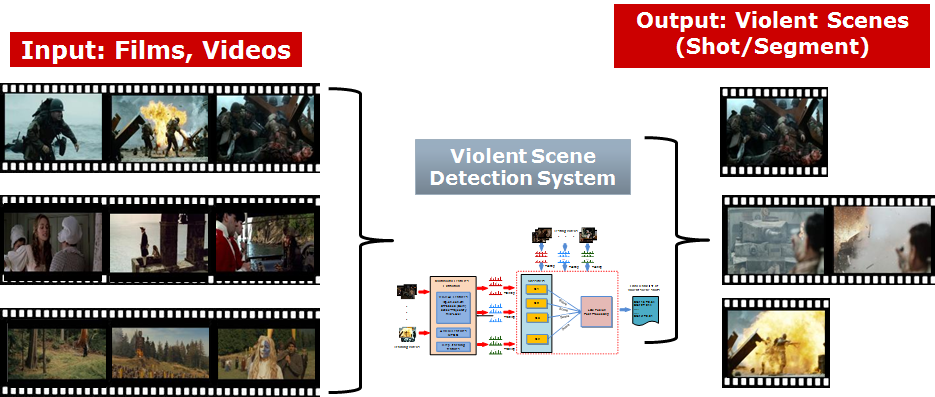
\includegraphics[width=1\linewidth]{Images/SystemOverview.png}
	\caption{Overview of violent scene detection system.}
	\label{fig:systemoverview}
\end{figure}

%In typical violent scene detection system (Figure~\ref{fig:systemoverview}), a user submits a movie and system will return shots or segments that include violent information. A general framework to build a such system usually consists of 4 components: shot segmentation, feature extraction, learning model, prediction. Firstly, the input movie is divided into fundamental video units or shots, then sampling keyframes are extracted for each shot; secondly, system extracts large array of multi features at multiple granularities; thirdly, multi violent classifiers are built from different features; finally, score fusion combines multiple scores which are predicted by classifiers and improves the overall performance. Most of existing approaches for similar system (such as multimedia event detection, action recognition, scene classification) focus on feature extraction component. The main observation drawn from these approaches is how to select the best features and combine of multi features to handle large variations of violent scenes. 

Given a movie as input, the expected output of a VSD system is all shots and segments having violent information. A general framework contains 4 main processing steps: video segmentation, feature extraction, learning models, and prediction. In the first step, the input movie is divided into fundamental processing units i.e. video shots. Then, features are extracted from the shots in second step. The goal of this step is to extract meaningful features which will be used for learning and predicting concepts in shots in later steps. Related studies for similar system (e.g. multimedia event detection, action recognition, scene classification) have shown that selecting relevant features and their combination is essential for accurate detection.
\begin{figure}[!t]
	\centering
	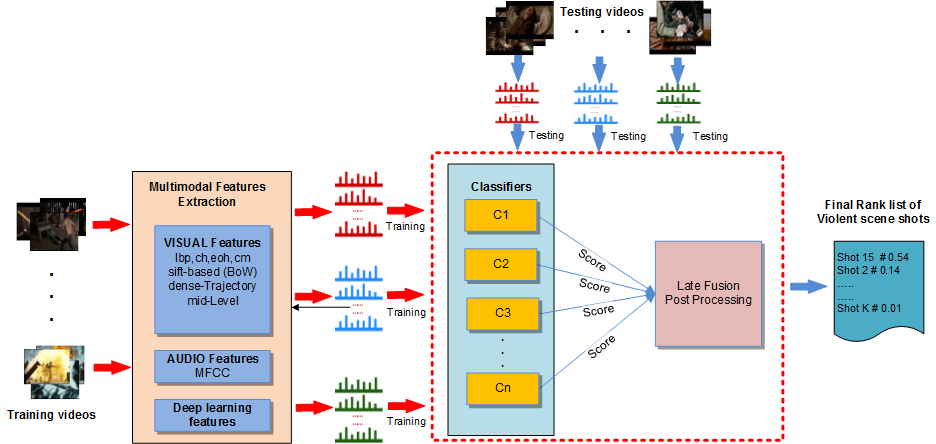
\includegraphics[width=1\linewidth]{Images/Framework1.png}
	\caption{Overview of violent scene detection framework.}
	\label{fig:framework}
\end{figure}

%In this paper, we present a framework that is designed to evaluate every single type of features and incorporate multi features for VSD. Figure~\ref{fig:framework} shows our system architecture.  We extracted visual (image and video), audio and deep learning features. Visual features are proposed to describe visual characteristics of violent concept, such as the objects, the scenes. Audio feature is used to capture the sound of violent actions. In addition, motion feature is used describe the actions, the activities. We rigorously analyze and combine a set of low-level features that capture violent appearance in video shots. We also evaluate the utility of mid-level representation to reduce the semantic gap between violence concept and low-level features. “Mid-level” means this layer lies between low-level features and high-level target events. Further, we investigate how to combine these diverse features using several fusion methods to improve overall performance of system. The main focus of this work is to provide a comparative analysis of value of multi features for VSD. Our study is helpful in that it evidences strong and weak points of current violence detection techniques and can be used to guide further work in the area.

In this paper, we evaluate various types of features and their combinations for VSD. 
\begin{itemize}
	\item {\bf Visual features:} are proposed to describe visual characteristics of violent concept, such as the objects, the scenes. We evaluate color moments, color histogram, edge orientation histogram, and local binary patterns, SIFT, Color-SIFT, Opponent-SIFT.
	\item {\bf Audio feature:} is used  to capture the sound of violent actions. We use MFCC feature.
	\item {\bf Visual motion feature:} is used to describe the actions, the activities. We use Dense Trajectory feature with Motion Boundary Histogram (MBH), Histograms of Oriented Gradients (HoG),  Histograms of Optical Flow (HoF) as feature descriptors.
	\item {\bf Mid-level feature:} is used to narrow the semantic gap between visual local features and violent concept.
\end{itemize}
The main focus is to provide a comparative analysis on features and their contributions to the final performance of a VSD system. The observation drawn from our work may be helpful to future works in the field.

We perform our experiments of a standard benchmark, MediaEval VSD 2014\cite{demarty2014benchmarking} which are made publicly available \footnote{http://www.technicolor.com/en/innovation/research-innovation/scientific-data-sharing/violent-scenes-dataset} . Our system is trained and tested on Hollywood movies within MediaEval VSD Dataset and evaluated by MediaEval VSD official metric (MAP-mean average precision). By using this standard dataset and evaluation protocol makes our proposed methods to be fair to compare with results by other MediaEval VSD participants (results did not use the external data). Results show the performance of visual features are the best. Low-level visual features and motion feature play very important role when fusing all modalities. Audio and mid-level features are not good as low-level visual features but they are complementary to improve overall performance. Experiments with several fusion methods show that all single features are complementary and help to improve overall performance.

The rest of this paper is organized as follows. We review some related work in section 2. Section 3 introduces our framework, our approaches for feature extraction, and detail of feature configurations, fusion methods. The experimental results and their analysis will be in section 4, as well as the conclusion and future works are described in the section 5 of this paper.
\section{Related work}
Violent scene detection is a kind of multimedia event detection. Although combining multiple features from multi-modalities has been proven as an effective strategy for multimedia event detection, relatively few works have been proposed to apply these approaches for violent scene detection in video. The main reason is that the definition of violence is ambiguous. It is difficult to describe this high-level concept using mathematical formulation precisely. In general, the violence concept is not well-defined and recent approaches addressed the problem by their own definitions.

Some of the previous works applied different kind of visual features to detect flame, blood, explosion as the informative cues for violence. As a first approach in this field, Jeho \cite{nam1998audio} propose an approach to recognize violent scenes in videos by detecting flame and blood, capturing the degree of motion activity, the soundtrack and characterization of sound effects of violent events. Meanwhile, Chen \cite{2} decompose violent scene detection into action scene detection and bloody frame detection. Clarin \cite{3} present a system which uses a Kohonen self-organizing map, which is for detecting skin and blood pixels in each frame, and motion intensity analysis to detect violent actions involving blood. More recently, Gong Yu \cite{11} introduce a violence detector using low-level visual and auditory features and high-level audio effects to identify potential violent content in movies. Jian \cite{17} describe a weakly-supervised audio violence classifier combined using co-training with a motion, explosion and blood video classifier to detect violent scenes in movies. Penet \cite{21} compared two modality fusion methods, namely Early Fusion and Late Fusion. Early Fusion concatenates features from both modalities before machine learning, while Late Fusion fuses probabilities of both modalities already calculated. They reported Late Fusion was superior to Early Fusion.

Beside low-level based approaches, violent scene detection is also a kind of high level recognition task. The major challenge is to deal with the gap of semantic meaning. In recent years, there are some approaches using attributes to narrow the semantic gap in high-level recognition task, such as object recognition using attributes, scene classification using attributes, action recognition using actions bank\cite{23}. Li \cite{15} propose ”Object Bank” (OB), a new representation of natural images based on objects (using objects as attributes to describe scenes). Liu \cite{18} use high-level semantic concepts, also called attributes, to represent human actions from videos and argue that attributes enable the construction of more descriptive models for human action recognition. Sasanand \cite{23} present Action Bank”, a new high-level representation (kind of attributes) of video.  For VSD, Bodgan \cite{13} rely on fusing mid-level concept predictions made using multi-layer perception classifiers to automatically localize the occurrence of violence within a video.  They proposed a frame-level violence prediction, applying a multi-layer perceptron in order to utilize these concepts. They put the first layer for the concept prediction, and the second layer for the violence prediction. In addition to those provided concepts, Tan \cite{tan2013vireo} have utilized extra 42 violence concepts such as bomb and war from ConceptNet\cite{liu2004conceptnet}. ConceptNet is composed of nodes representing concepts in the form of words or short phrases with their relationships. On their system those extra concepts are trained using YouTube videos which are crawled additionally. 

In the last few years, MediaEval Violent Scene Detection affect Task is become popular, many state-of-the art systems have been developed and reported recently\cite{demarty2014benchmarking}. Most systems extract a large number of multimodal features from visual, audio signals and text.  The features include low-level features such as color histogram, edge of histogram, local binary pattern, SIFT based, Space-Time Interest Points (STIP), Histograms of Oriented Gradients (HoG), Histograms of Optical Flow (HoF), Motion Boundary Histograms (MBH), visual activity, MFCCs, trajectory-based features  (cite each team). Different state-of-the-art features encoding are used, such as Bag-of-Visual-Words representation, Fisher vector representations. In addition, some approaches use of pre-defined concept detectors like part-level attributes – FUDAN Team\cite{dai2013fudan}, mid-level concept description, with provided concepts from ConceptNet (e.g., punishment, victim, rape, etc) – VIREO team\cite{tan2013vireo}. The video shots are classified by using different machine learning techniques (Support Vector Machines (SVMs), k nearest neighbors (kNN), Bayesian Network). Multimodal integration is achieved via early fusion\cite{penet2013technicolor}  and late fusion\cite{penet2013technicolor,sjoberg2013far,derbas2013lig,dai2013fudan} where score fusion is often used to combine scores independently computed from different subsets of features.

In this paper, we present a novel violent scene detection framework which is designed to incorporate many of the above-mentioned success principles in its architecture. In particular, our work incorporates novel developments into the system, which can be summarized into major contributions. First, our work developed and incorporated multi modal features at diverse granularities to evaluate the value of different types of features for VSD. Second, our work explores the use of mid-level concept features, which are detected based on low-level features, aiming to provide more semantic understanding capability into our system. Third,  we present several approaches to learn fusion functions which combine violent scores (late fusion) to improve overall performance.

\section{VSD system}
\subsection{Framework Overview}
We use a unified framework to evaluate the performance of each feature as well as the performance of feature combination methods. The framework should be flexible so that we can easily test different kind of features or fusion strategies. It also should be designed in a component-based manner so that we can evaluate each component separately while keeping other components intact. In this spirit, our framework can be decomposed into following components: (1) Pre-processing, (2) Feature Extraction, (3) Feature Encoding, (4) Feature Classification and (5) Feature Fusion. The detail of each component is described in the following sections. We especially focus on the feature encoding and feature fusion component. The former is used to evaluate features while the later is used to evaluate fusion strategies for VSD. An overview of our framework is shown in Figure \ref{fig:framework}.

\subsection{Pre-processing}
%\subsection{Keyframe Extraction and Shot Pooling}
To create a feature representation for each shot: firstly, we extract five keyframes per second; secondly, we extract visual feature for each keyframe; lastly, we apply maximum and average pooling methods to create shot-based features.
\subsection{Feature Extraction}
The feature extraction component aims to make a discriminative vector representation for each shot that is extracted from the pre-processing step. The extraction method depends on what type of feature will be used. To conduct a comprehensive evaluation of features for VSD, we support a large variety of features including global and local visual features. Global features capture the global statistics of each extracted shot. These statistics can be calculated directly from sub regions of a sampled frame and then concatenated to form the vector representation for that frame, before being aggregated to make the final representation for each shot. It is more complicated to calculate the feature vector representation for local features. The number of local features vary from frame to frame, therefore it requires a special encoding technique which will be described in \ref{feature_encoding}.

Besides global and local features, other features are also supported in our evaluation framework. Audio feature can be extracted from pre-defined temporal windows. Feature of each temporal window provide a local audio characteristic at that temporal location. Therefore, audio feature can be considered as a local feature and can be well-integrated into our feature extraction framework. Another feature that is also supported is mid-level feature, which is represented from violent concept detectors. We consider both the in-domain and out-domain concept detectors. In case the concepts are used from off-the-shelf datasets, we employ the state-of-the-art deep learning features which are extracted from a pre-trained model. The detail description of each feature is presented in Section \ref{vsd_feature}.

\subsection{Feature Encoding}
\label{feature_encoding}

%\subsection{Feature representation}

We employed the bag-of-words model with codebook size of 1000 and soft-assignment technique to generate a fixed-dimension feature representation for each keyframe. Besides encoding the whole image, we also divided it into grids of 3x1 and 2x2 to encode spatial information.
\begin{figure}[!h]
	\centering
	\includegraphics[width=0.7\linewidth]{Images/Bow.png}
	\caption{Bag of visual words.}
	\label{fig:bow}
\end{figure}
Besides the bag-of-words representation for the whole image, we divided each key frame into 2 \ding{53} 2 and 1 \ding{53} 3 sub-regions to cover information about the spatial layout of features, which is a trade off between performance and computation cost brought by the high dimensionality of the feature vector, and computed the bag-of-word representation for each sub-region. We applied this method for visual local features.
\subsection{Feature Classification}

%\subsection{Learning Classification}
LibSVM \cite{LibSVM} is used for training and testing at shot level. To generate training data, shots which fall into positive segments more than 80\% will be considered as positive shots. The remaining shots are considered as negative. Extracted features are scaled to [0, 1] using the svm-scale tool of LibSVM. We use chi-square kernel to calculate the distance matrix. The optimal (C;g) parameters for learning SVM classifiers are found by conducting a grid search with 5-fold cross validation on the original dataset.

\subsection{Feature Fusion}
\subsubsection{Late Fusion}
Fusing information coming from different media seems a natural way to handle multimedia content. Fusing of multi-modal information has been widely used for tasks including multimedia event detection, video search, etc. Naturally different semantic events, types of multimedia data have their own characteristics so their fusion strategies could be different also. For violent scene detection, we investigated several simple but effective fusion schemes to construct a better violence prediction system that exploits the advantages of each type of modalities. 

\section{VSD features}
\label{vsd_feature}

\subsection{Visual global features}

We evaluate both global features and local features. We selected the best configuration of each types of features from our previous work\cite{lam2012nii}. The global features include color moments, color histogram, edge orientation histogram, and local binary patterns with different configuration:

\begin{itemize}
	\item Granularity:  Since global features do not capture spatial information, to overcome this problem, a grid n×m usually used to divide the input image into non overlapping sub-regions. The features extracted from these regions are concatenated to form the feature vector for the image.
	\item Color space: Local binary patterns (LBP) and edge orientation histogram (EOH) are extracted from gray scale image. For color moments and color histogram, color spaces including HSV, RGB, Luv, and YCrCb are used.
	\item Quantization: For color histogram, we only use 8-bin histogram for each channel. For edge orientation histogram, we quantize orientations into histograms of 36 (edge) + 1(non-edge) bins. For local binary patterns, we quantize binary patterns into histograms of 30, 59 bins.
\end{itemize}

\subsection{Visual local features}
\subsubsection{Still image feature}

For local feature, we use popular SIFT with both Hessian Laplace interest points and dense sampling at multiple scales. For dense sampling, besides normal SIFT descriptor, we also use Opponent-SIFT and C-SIFT. For Harlap interest point detector, we only use normal SIFT descriptor.	

\subsubsection{Motion feature}
As shown by Wang et al. \cite{wang_dense}, Dense Trajectory feature is one of the best approaches for action classification. Dense Trajectory has an efficient solution to remove camera motion. In the Hollywood movies, there are a lot of action with different movie effects in the violent scenes. We try to apply the dense trajectory  to capture these information. Trajectories are obtained by tracking the densely sampled points in the optical flow fields. We use Motion Boundary Histogram (MBH) to describe each trajectory. This feature descriptor is good for handling camera motion. 
\subsubsection{Audio feature}
We use the popular MFCC for extracting audio feature. We choose the audio segment of 25ms and step size of 10ms. The 13d MFCCs along with each first and second derivatives are used for representing each audio segment. Raw MFCC features are also encoded using BoW. 

\subsection{Mid-level feature}
\subsubsection{In domain: VSD concepts}

Violent scene detection is also a kind of highlevel recognition task. Violence concept has high semantic meaning and high
variability in appearance. Besides that, due to lack of training data for this concept, training violence classifier directly
from low-level features is not effective. Instead of focusing on selecting the low-level features for VSD, we try to investigate how to use related violent information as mid-level feature to detect violent scene in the movie. We manually select the violent information which are annotated by human assessors as related attributes of violence concept.Then we propose to use such concepts as related semantic attributes of the original violence concept. Figure \ref{fig:exampleVS} shows how to describe the violent scene by their semantic attributes. These attributes which can be more well-presented by low-level features (e.g. the attribute about ”blood” can be sufficiently presented by color) are used to create the mid-level features. In other words, the attributes have smaller gap to the low-level features, compared to the original violence concept. For example, in Figure 1, because violence occurred during the whole scene, it is very hard to use low-level features to represent the violence concept. But, we can use the low-level visual features to represent some attributes such as “fire”, ”blood”. By doing this, we narrow the semantic gap between the original violence concept and low-level features extracted from video shots.
\begin{figure}[!t]
	\centering
	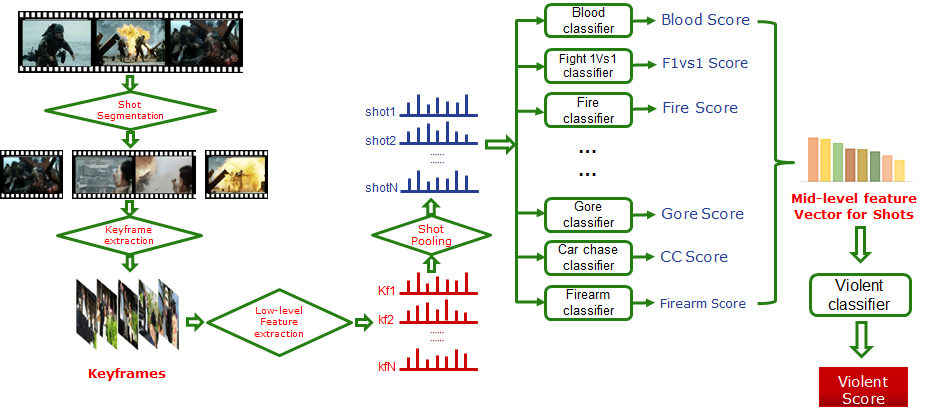
\includegraphics[width=1\linewidth]{Images/Mid-level.png}
	\caption{Overview of Mid-level framework.}
	\label{fig:mid-level}
\end{figure}
Attributes related to violence concept are manually defined. We used seven related concepts provided in MediaEval Dataset as violent attributes. Our mid-level framework is shown in Figure~\ref{fig:mid-level}. Firstly, each corresponding attribute classifier is trained by using low-level features. Secondly, the mid-level features of a training (or test) video shots are formulated by concatenating scores returned by attribute classifiers. At the moment, we use the same weights for concatenating different scores. Then thirdly, we use this feature to train the mid-level feature-based violence classifier.  Finally, we apply this violence classifier on test set to get the violence score for each shot (these shots are also represented by mid-level features).

\subsubsection{Out domain: Deep learning feature}

\section{Experiments}
\subsection{Dataset}
In this paper, we used the dataset from MediaEval  Affect Task 2014 \cite{demarty2014benchmarking}, this is a set of 31 Hollywood movies that must be purchased the original DVD due to copyright issues. The movies are of different genres (from extremely violence movies to movies without violence). In this dataset, we focus on the violent concept with subjective definition, which is defined as “those which one would not let an 8 years old child see because they contain physical violence”. Follow the proposed method, we divide this dataset into 2 parts:
\begin{table}[!t]
\begin{tabular}{ |p{0.05\textwidth} | p{0.5\textwidth} | p{0.25\textwidth} | p{0.1\textwidth} | p{0.1\textwidth} | }
	\hline
	No. & Video Name & Length (in second) & \# keyframes & \# shots \\ \hline
	1 & Armageddon-1998-dvd2002 & 8681.05 & 217026 & 1737 \\ \hline
	2 & BillyElliot-2000-dvd2003 & 6349.36 & 158734 & 1270 \\ \hline
	3 & Eragon-2006-dvd2007 & 5985.57 & 149639 & 1198 \\ \hline
	4 & HarryPotter5-2007-dvd2008 & 7954.72 & 198868 & 1591 \\ \hline
	5 & IAmLegend-2007-dvd2010 & 5780.58 & 144514 & 1157 \\ \hline
	6 & Leon-1994-dvd2004 & 6344.49 & 158612 & 1269 \\ \hline
	7 & MidnightExpress-1978-dvd2008 & 6960.96 & 174024 & 1393 \\ \hline
	8 & PiratesOfTheCaribbean1-2003-dvd2006 & 8241.01 & 206025 & 1649 \\ \hline
	9 & ReservoirDogs-1992-dvd2004 & 5712.98 & 142825 & 1143 \\ \hline
	10 & SavingPrivateRyan-1998-dvd2006 & 9750.89 & 243772 & 1951 \\ \hline
	11 & TheSixthSense-1999-dvd2000 & 6178.01 & 154450 & 1236 \\ \hline
	12 & TheWickerMan-2006-dvd2008 & 5870.89 & 146772 & 1175 \\ \hline
	13 & TheBourneIdentity-2002-dvd2006 & 6816.29 & 170407 & 1364 \\ \hline
	14 & TheWizardofOz-1939-dvd2000 & 5859.29 & 146482 & 1172 \\ \hline
	15 & DeadPoetsSociety-1989-dvd2002 & 7415.17 & 185379 & 1484 \\ \hline
	16 & FightClub-1999-dvd2001 & 8006.34 & 200158 & 1602 \\ \hline
	17 & IndependenceDay-1996-dvd2010 & 8834.96 & 220874 & 1767 \\ \hline
	18 & TheGodFather-1972-dvd2008 & 10194.96 & 254874 & 2039 \\ \hline
	19 & PulpFiction-1994-dvd2009 & 8887.97 & 222199 & 1778 \\ \hline
	20 & ForrestGump-1994-dvd2006 & 8176.97 & 204424 & 1636 \\ \hline
	21 & Fargo-1996-dvd2004 & 5646.34 & 141158 & 1130 \\ \hline
	22 & ThePianist-2002-dvd2007 & 8567.1 & 214177 & 1714 \\ \hline
	23 & FantasticFour1-2005-dvd2005 & 6094.41 & 152360 & 1219 \\ \hline
	24 & LegallyBlond-2001-dvd2002 & 5523.49 & 138087 & 1105 \\ \hline
	   & Total & 173833.8 & 4345840 & 34779 \\ \hline
\end{tabular}
\caption{DEVEL set includes 24 Hollywood movies.}
\label{devel-dataset}
\end{table}
\begin{table}[!t]
\begin{tabular}{ |p{0.05\textwidth} | p{0.5\textwidth} | p{0.25\textwidth} | p{0.1\textwidth} | p{0.1\textwidth} | }
	\hline
	No. & Video Name & Length (in second) & \# keyframes & \# shots \\ \hline
	1 & V\_FOR\_VENDETTA & 7626.49 & 190662 & 1526 \\ \hline
	2 & TERMINATOR\_2 & 8831.37 & 220784 & 1767 \\ \hline
	3 & JUMANJI\_COLLECTORS\_EDITION & 5993.98 & 149849 & 1199 \\ \hline
	4 & GHOST\_IN\_THE\_SHELL & 4966 & 124150 & 994 \\ \hline
	5 & DESPERADO & 6012.89 & 150322 & 1203 \\ \hline
	6 & BRAVEHEART & 10224.49 & 255612 & 2045 \\ \hline
	7 & 8\_MILE & 6355.53 & 158888 & 1272 \\ \hline
	  & Total & 50010.75 & 1250267 & 10006 \\ \hline
\end{tabular}
\caption{TEST set includes 7 Hollywood movies.}
\label{test-dataset}
\end{table}

\begin{itemize}
	\item DEVEL (Table~\ref{devel-dataset}): this is training dataset; used to train violence classifiers; has 24 movies, total 34779 shots, 48.29 hours. 
	\item TEST (Table~\ref{test-dataset}): this is testing dataset; used to test and evaluate the system; has 7 movies, total 10006 shots and 13.89 hours.
\end{itemize}
Total duration are about 62.18 hours, with 44.785 shots. To reduce the computation cost, when we extract keyframes, we resize the keyframes to 500x400 pixels.
\subsection{Groundtruth}
By using subjective definition in MediaEval VSD 2014\cite{demarty2014benchmarking}, the ground truth is created by human assessors and provided by the MediaEval organizers. In addition to segments containing physical violence, annotations also include the following high-level concepts: presence of blood, fights, presence of fire, presence of guns, presence of cold arms, car chases and gory scenes, for the visual modality; gunshot, explosion and scream for the audio modality. The ground truth data are provides in segment. To generate training data, we consider the positive shots are the ones which have 80\% overlapping with ground truth segments.
\subsection{Evaluation Metrics}
We use mean average precision (mAP), an evaluation metric that is widely used for classification and retrieval systems. The mAP is computed based on the ranked list of shots returned by the detection system and the ground truth provided by the task organizers. Mean average precision (mAP) is calculated as below:
\[
MAP=\ \frac{\sum_{v=1}^VAP(v)}{V}
\]
, where V is number of test videos and AP is average precision for each video.
\subsection{Results and comparison}
\subsubsection{Evaluation of global features}
\subsubsection{Evaluation of local features}
\subsubsection{Evaluation of motion features}
\subsubsection{Evaluation of audio features}
\subsubsection{Evaluation of mid-level features}
\subsubsection{Evaluation of deep learning features}
\subsubsection{Evaluation of fusion schema}
\subsubsection{Comparison with MediaEval teams}
\section{Conclusion}
We evaluate the performance of multi features for the violent scene detection. The performance of global features and local features that are widely used in state of the art classification systems are compared. Our study can be served as a baseline for comparison of advanced algorithms or systems in the violent scene detection. Still image based feature (SIFT) has better performance than motion based feature (Dens-trajectory + MBH).  Fusion of global features is effective, while fusion of local features is not (only SIFT is enough). Fusion of local features, global features, motion features and audio feature achieves the best performance. Post-processing method is very effective to improve overall performance. Mid-level representation shows promising results compared to using raw feature only, however the performance is still limited. But adding mid-level feature in fusion schema is not effective. Experimental results on MediaEval 2013 VSD benchmark dataset show the validity of the approach and its comparable performance to state-of-the-art methods.

\section*{References}

\bibliography{mybibfile}

\end{document}